\documentclass[11pt]{article}
\usepackage[utf8]{inputenc}
\usepackage{xcolor, comment, subfiles, graphicx, caption, longtable, subfig, fancyhdr}
\usepackage{float} %Used to force images to appear in the section in which it's declared
\usepackage[hidelinks]{hyperref}
\usepackage{parskip}
\usepackage[shortlabels]{enumitem}
\usepackage{multirow}
\usepackage{color}
\usepackage[toc,page]{appendix}
\usepackage{float}
\usepackage[a4paper,width=150mm,top=25mm,bottom=25mm]{geometry}
\usepackage{longtable}
\usepackage{colortbl}
\usepackage{xcolor}
\usepackage{color}
\usepackage{amsfonts}
\usepackage{amssymb}
\usepackage{amsmath}
\usepackage{cancel}


\newcommand{\subf}[2]{%
  {\small\begin{tabular}[t]{@{}c@{}}
   \mbox{}\\[-\ht\strutbox]
   #1\\#2
   \end{tabular}}%
}

\title{DASA - Project}
\makeatletter

\begin{document}

\setlength{\parskip}{1em}

\begin{titlepage}
\centering
\vfill
{

\includegraphics[width =\linewidth, height = 4cm, keepaspectratio]{PolitecnicoLogo.png}
\label{fig:PolitecnicoLogo}
\large \\[2ex]M.Sc. Computer Science and Engineering\\
\large Data Analysis for Smart Agriculture\\[12ex]
\huge
Data Analysis On An Eggs Farm\\[1.5ex]
\large
\vspace{10mm}

\vspace{15mm}
\normalsize

\vspace{30mm}

\begin{tabular}{lclcl}
    Davide Canali & - & 10674880 & - & davide1.canali@polimi.it\\
    Matteo Cordioli & - & 10611332 & - & matteo.cordioli@mail.polimi.it\\
    Federico Camilletti & - & 10619856 & - & federico.camilletti@mail.polimi.it\\
    Shakiba Shahidiani  & - & 00000000 & - & shakiba.shahidiani@mail.polimi.it\\
\end{tabular}

\vspace{30mm}

\@date\\[2.5ex]
}
\end{titlepage}

\makeatother
\tableofcontents
\newpage

\section{Introduction}
In this study, we will expose the data analysis done starting from data gathered from an eggs farm near Mantova to see if it's possible to improve both animal welfare and farmer revenue.

The farm under analysis is "Boccola Allevamenti Avicoli Soc Agricola SS" and has around 40'000 chickens that produce organic eggs. They provided us with data starting from 2014, the production of eggs is divided into cycles lasting about 13 - 15 months each. The analysis will consider 5 complete cycles and the current 2022 cycle. The first 2 cycles (called X and Y) are non-organic which means the chickens are treated differently from the last 4 cycles (Z, A, B, C) which are organic.

The chickens are divided into 2 equal-sized barns, both of which receive the same treatment and operations.

The farmer is in an agistment that takes care of refurbishing the feed and the livestock.

Upon talking with the farmer we focus our attention on 3 main topics which involve:
\begin{itemize}
    \item Understanding the mortality between different cycles and organic with non-organic.
    \item Improve the welfare of the chickens.
    \item Quantify the monetary loss when a chicken dies at the start of the cycle. //TODO
    \item Quantify the losses in cycle C
\end{itemize}

\section{Data}
\subsection{Data Collection}
The farmer collected the data thanks to sensors and by inspecting the barns each day. Before cycle A the data were only collected in paper spreadsheets and to be used were needed to be imported in a digital format.
The data on paper had 5 features: date, death, current chickens, eggs produced and sold
when the data became saved digitally 2 extra features were collected which are feed and water.

\subsection{Data Cleaning}
Before starting to analyze the data we cleaned them.
In all the cycles we performed these next steps:
\begin{itemize}
    \item Removed tail and head (20 rows each more or less).
    \item Adjusted feed and water consumption to correct typos and switchboard errors.
    \item Adjusted eggs production when \% of laid when above 100\%, distributed in the days before assuming that those eggs were not collected.
    \item Adjusted death count to match the delta of death at the end of the cycle.
    \item Checked that the difference between the total amount of eggs produced and the number of eggs sold was less than 0.6\%.
\end{itemize}

Specifically, in cycle A we also adjust a series of missing data regarding the water consumption adding them following the cycle distribution.
Cycles X and Y needed some normalization in the amount of eggs per day, many days had the exact same amount of eggs, which is statistically impossible. Talking with farmers we understand that were numbers placed for easyness to sell the eggs, a replacing of all those number were needed. We replaced the value of those days with the avarage of the 7 days before.



\section{Analysis of Each Cycle}
\subsection{Clustering Techniques}
We used 3 different clustering techniques K-Means, Hierarchical and Density Based Clustering.
To choose the parameters for these methods we used different solutions:
\begin{itemize}
    \item K-Means: silhouette technique to find the optimal number of clusters.
    \item Hierarchical: plot the dendrogram to find the optimal number of clusters.
    \item Density: plot the k-NN to find the optimal $\epsilon$.
\end{itemize}
\subsection{Cycle A}
\begin{center}
    \begin{tabular}{|c | c | c | c | c | c|} 
        \hline
        \textbf{Arrival date} & \textbf{\#Chickens} & \textbf{Frist Laid} & \textbf{End of cycle} & \textbf{Organic} & \textbf{\#Eggs}\\ [0.5ex] 
        \hline
        19/7/2018 & 42.009 & 1/9/2018 & 19/5/2020 & Yes & 20.208.086\\
        \hline
    \end{tabular}
\end{center}
Significant features:
\begin{itemize}
    \item Average Percentage of Laid Eggs each day: 83,8\%
    \item Average Percentage of Death each day: 0,044\%
    \item Average Temperature during the cycle: 12,99 °C
    \item Average Humidity during the cycle: 74,55\%
\end{itemize}

Cluster:
\begin{center}
\begin{tabular}{|c|c|}
    \hline
    \subf{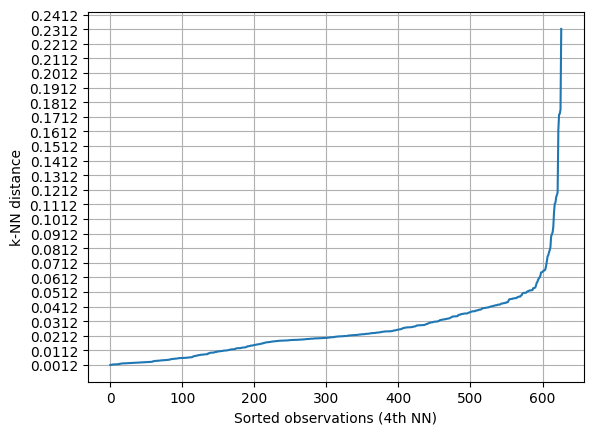
\includegraphics[width=70mm]
    {../Results/Two_clusters_division/CycleA/Density_epsilon.png}}
         {k-NN distance to find $\epsilon$}
    &
    \subf{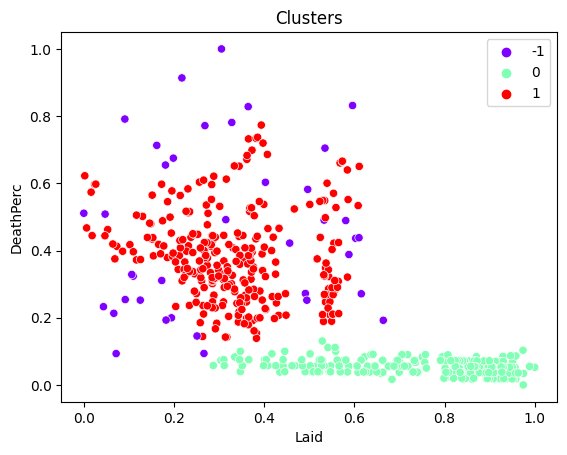
\includegraphics[width=70mm]
    {../Results/Two_clusters_division/CycleA/Density_scatter_merged.png}}
         {Density scatter plot merged}
    \\
    \hline
    \subf{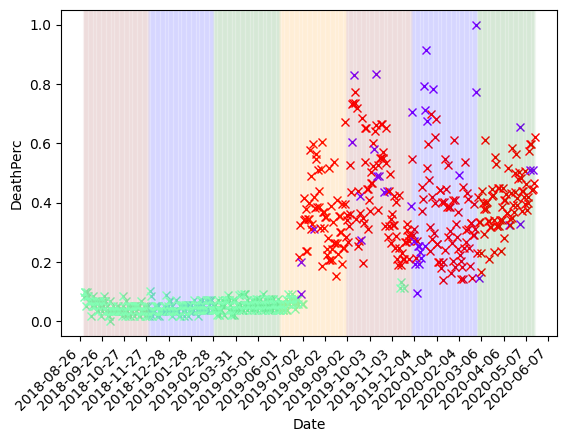
\includegraphics[width=70mm]
    {../Results/Two_clusters_division/CycleA/Density_plot_death.png}}
         {Percentage of death}
    &
    \subf{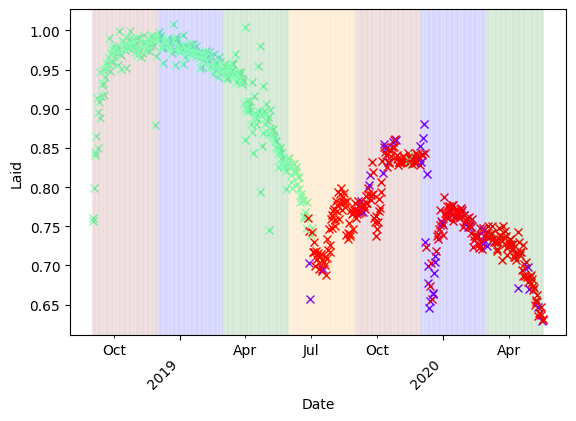
\includegraphics[width=70mm]
    {../Results/Two_clusters_division/CycleA/Density_plot_laied.png}}
         {Percentage of laid eggs}
    \\
    \hline
\end{tabular}
\end{center}

\subsection{Cycle B}
\begin{center}
    \begin{tabular}{| c | c | c | c | c | c | c |} 
        \hline
        Arrival date & \#Chickens & Frist Laid & End of cycle & Organic & \#Eggs\\ [0.5ex] 
        \hline
        09/08/2020 & 42.098 & 24/09/2020 & 02/05/2022 & Yes & 18.392.640\\ 
        \hline
    \end{tabular}
\end{center}

Significant features:
\begin{itemize}
    \item Average Percentage of Laid Eggs each day: 81,39\%
    \item Average Percentage of Death each day: 0,0494\%
    \item Average Temperature during the cycle: 11,81 °C
    \item Average Humidity during the cycle: 73,24\%
\end{itemize}

Cluster:
\begin{center}
\begin{tabular}{|c|c|}
    \hline
    \subf{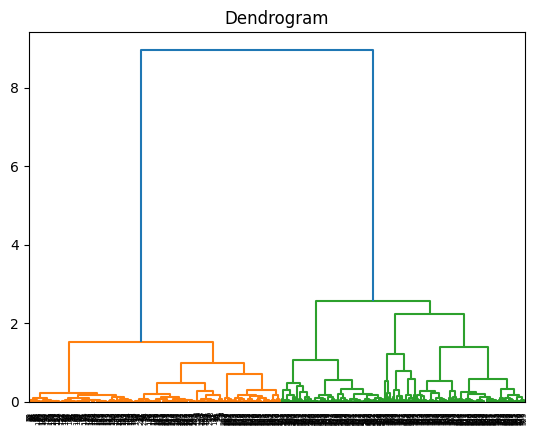
\includegraphics[width=70mm]
    {../Results/Two_clusters_division/CycleB/Hierarchical_dendogram.png}}
         {Dendrogram}
    &
    \subf{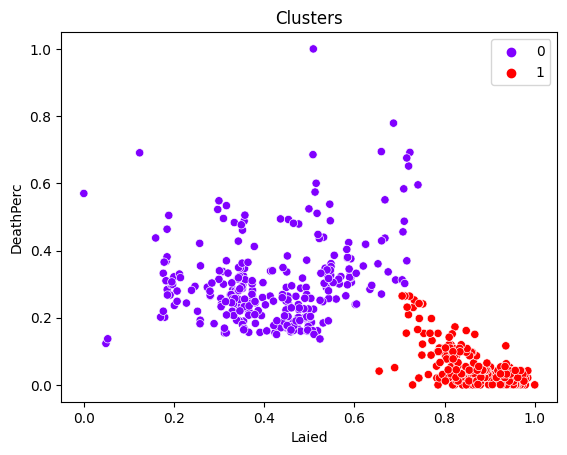
\includegraphics[width=70mm]
    {../Results/Two_clusters_division/CycleB/Hierarchical_scatter.png}}
         {Hierarchical cluster scatter plot}
    \\
    \hline
    \subf{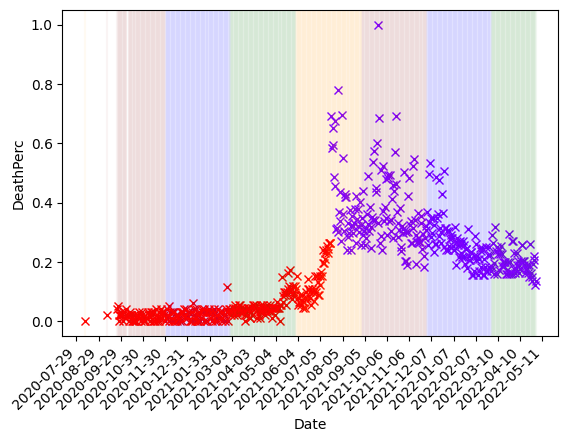
\includegraphics[width=70mm]
    {../Results/Two_clusters_division/CycleB/Hierarchical_plot_death.png}}
         {Percentage of death}
    &
    \subf{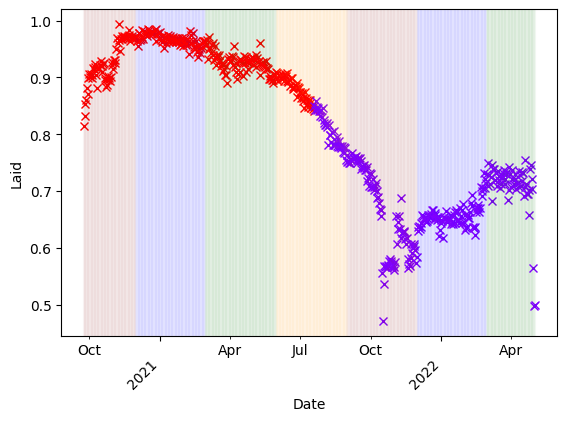
\includegraphics[width=70mm]
    {../Results/Two_clusters_division/CycleB/Hierarchical_plot_laied.png}}
         {Percentage of laid eggs}
    \\
    \hline
\end{tabular}
\end{center}

\subsection{Cycle C}
\begin{center}
    \begin{tabular}{| c | c | c | c | c | c | c |} 
        \hline
        Arrival date & \#Chickens & Frist Laid & End of cycle & Organic & \#Eggs\\ [0.5ex] 
        \hline
        20/06/2022 & 42.098 & 08/08/2022 & In progress & Yes & In progress\\ 
        \hline
    \end{tabular}
\end{center}

Significant features:
\begin{itemize}
    \item Average Percentage of Laid Eggs each day: 55,85\%
    \item Average Percentage of Death each day: 0,043\%
    \item Average Temperature during the cycle: 18,61 °C
    \item Average Humidity during the cycle: 70,05\%
\end{itemize}

Cluster:
\begin{center}
\begin{tabular}{|c|c|}
    \hline
    \subf{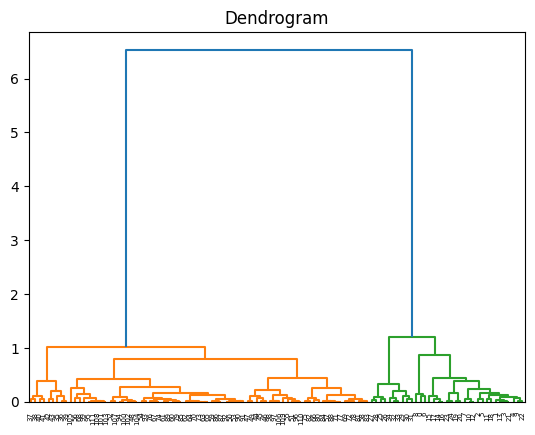
\includegraphics[width=70mm]
    {../Results/Two_clusters_division/CycleC/Hierarchical_dendogram.png}}
         {Dendrogram}
    &
    \subf{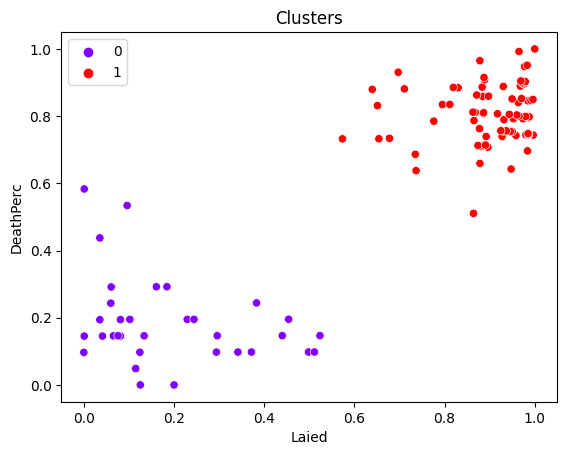
\includegraphics[width=70mm]
    {../Results/Two_clusters_division/CycleC/Hierarchical_scatter.png}}
         {Hierarchical cluster scatter plot}
    \\
    \hline
    \subf{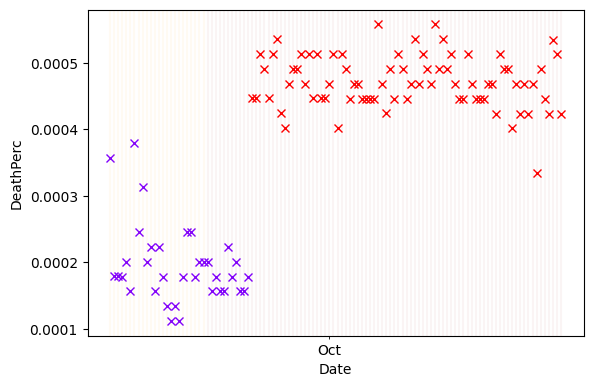
\includegraphics[width=70mm]
    {../Results/Two_clusters_division/CycleC/Hierarchical_plot_death.png}}
         {Percentage of death}
    &
    \subf{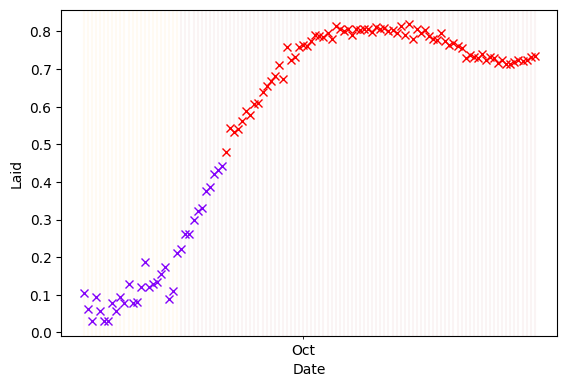
\includegraphics[width=70mm]
    {../Results/Two_clusters_division/CycleC/Hierarchical_plot_laied.png}}
         {Percentage of laid eggs}
    \\
    \hline
\end{tabular}
\end{center}

\subsection{Cycle X1}
\begin{center}
    \begin{tabular}{| c | c | c | c | c | c | c |} 
        \hline
        Arrival date & \#Chickens & Frist Laid & End of cycle & Organic & \#Eggs\\ [0.5ex] 
        \hline
        20/01/2014 & 33.743 & 18/03/2014 & 08/07/2015 & No & 12.375.840\\ 
        \hline
    \end{tabular}
\end{center}

Significant features:
\begin{itemize}
    \item Average Percentage of Laid Eggs each day: 80,69\%
    \item Average Percentage of Death each day: 0,032\%
    \item Average Temperature during the cycle: 15,34 °C
    \item Average Humidity during the cycle: 72,83\%
\end{itemize}

Cluster:
\begin{center}
\begin{tabular}{|c|c|}
    \hline
    \subf{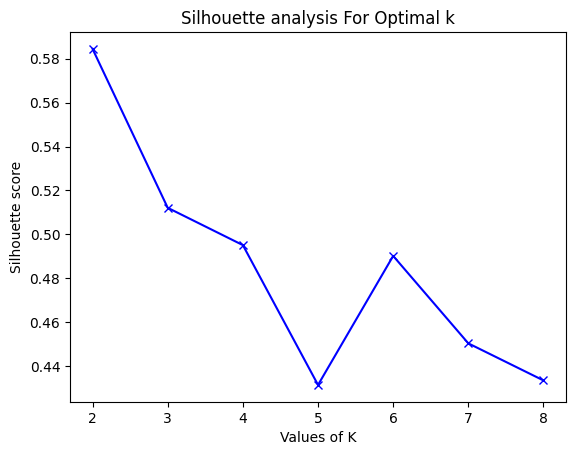
\includegraphics[width=70mm]
    {../Results/Two_clusters_division/CycleX1/KMeans_silhouette.png}}
         {Silhouette}
    &
    \subf{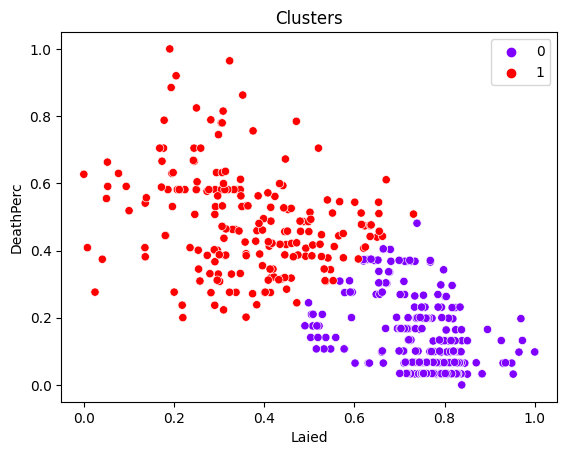
\includegraphics[width=70mm]
    {../Results/Two_clusters_division/CycleX1/KMeans_scatter.png}}
         {K-Means cluster scatter plot}
    \\
    \hline
    \subf{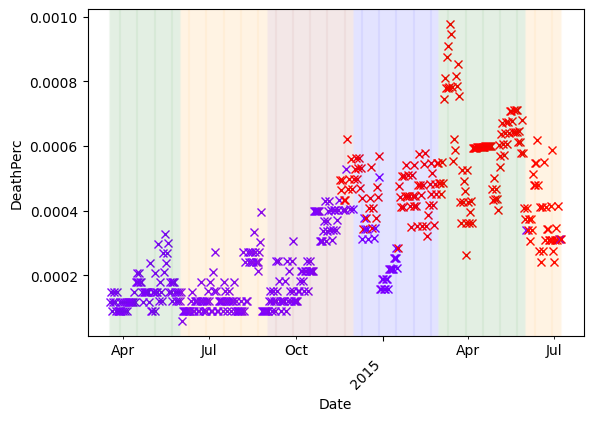
\includegraphics[width=70mm]
    {../Results/Two_clusters_division/CycleX1/KMeans_plot_death.png}}
         {Percentage of death}
    &
    \subf{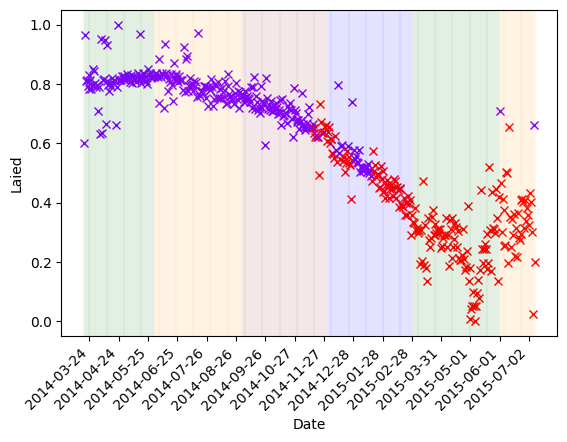
\includegraphics[width=70mm]
    {../Results/Two_clusters_division/CycleX1/KMeans_plot_laied.png}}
         {Percentage of laid eggs}
    \\
    \hline
\end{tabular}
\end{center}

\subsection{Cycle X2}
\begin{center}
    \begin{tabular}{| c | c | c | c | c | c | c |} 
        \hline
        Arrival date & \#Chickens & Frist Laid & End of cycle & Organic & \#Eggs\\ [0.5ex] 
        \hline
        26/05/2014 & 23.898 & 15/07/2014 & 21/06/2015 & No & 7.558.799\\ 
        \hline
    \end{tabular}
\end{center}

Significant features:
\begin{itemize}
    \item Average Percentage of Laid Eggs each day: 95,36\%
    \item Average Percentage of Death each day: 0,021\%
    \item Average Temperature during the cycle: 13,76 °C
    \item Average Humidity during the cycle: 76,04\%
\end{itemize}

Cluster:
\begin{center}
\begin{tabular}{|c|c|}
    \hline
    \subf{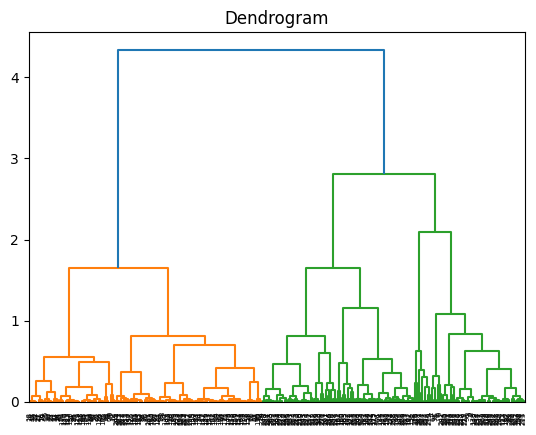
\includegraphics[width=70mm]
    {../Results/Two_clusters_division/CycleX2/Hierarchical_dendogram.png}}
         {Dendrogram}
    &
    \subf{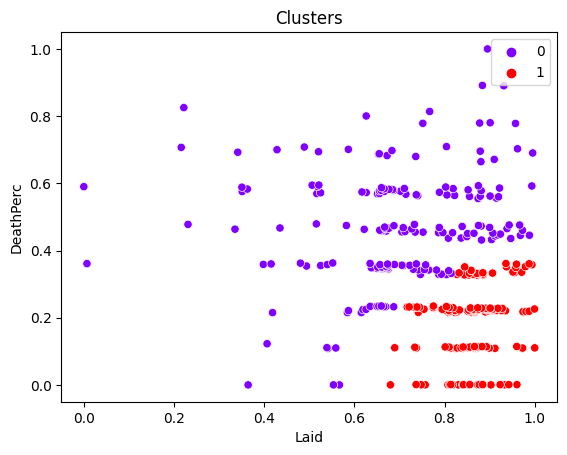
\includegraphics[width=70mm]
    {../Results/Two_clusters_division/CycleX2/Hierarchical_scatter.png}}
         {Hierarchical cluster scatter plot}
    \\
    \hline
    \subf{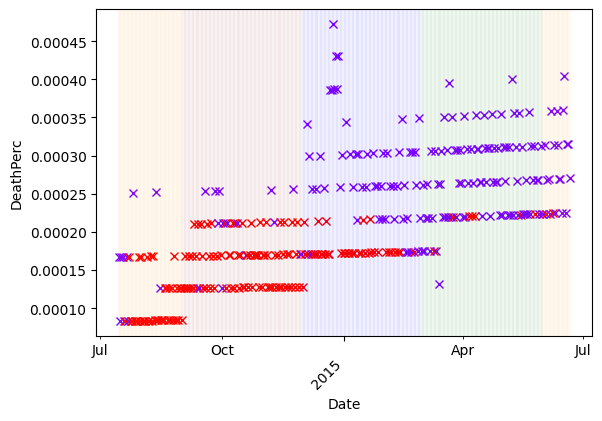
\includegraphics[width=70mm]
    {../Results/Two_clusters_division/CycleX2/Hierarchical_plot_death.png}}
         {Percentage of death}
    &
    \subf{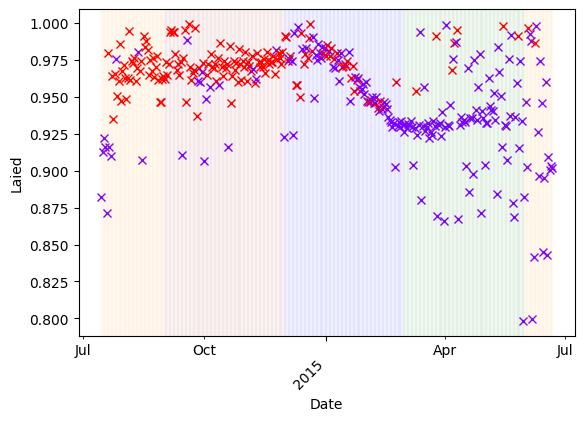
\includegraphics[width=70mm]
    {../Results/Two_clusters_division/CycleX2/Hierarchical_plot_laied.png}}
         {Percentage of laid eggs}
    \\
    \hline
\end{tabular}
\end{center}

\subsection{Cycle Y}
\begin{center}
    \begin{tabular}{| c | c | c | c | c | c | c |} 
        \hline
        Arrival date & \#Chickens & Frist Laid & End of cycle & Organic & \#Eggs\\ [0.5ex] 
        \hline
        11/08/2015 & 57.346 & 05/10/2015 & 27/09/2016 & No & 16.759.240\\ 
        \hline
    \end{tabular}
\end{center}

Significant features:
\begin{itemize}
    \item Average Percentage of Laid Eggs each day: 83.70\%
    \item Average Percentage of Death each day: 0,022\%
    \item Average Temperature during the cycle: 14,20 °C
    \item Average Humidity during the cycle: 74,54\%
\end{itemize}

Cluster:
\begin{center}
\begin{tabular}{|c|c|}
    \hline
    \subf{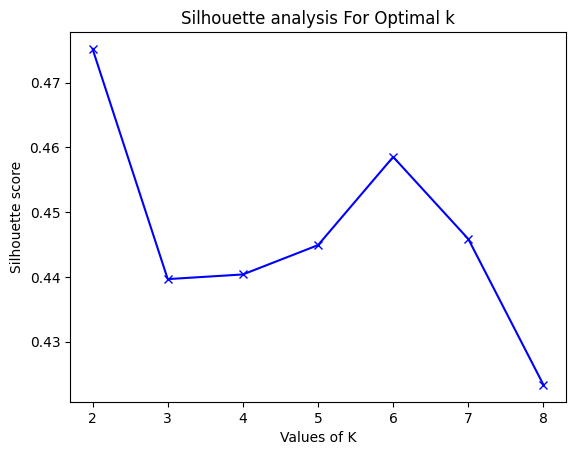
\includegraphics[width=70mm]
    {../Results/Two_clusters_division/CycleY/KMeans_silhouette.png}}
         {Silhouette}
    &
    \subf{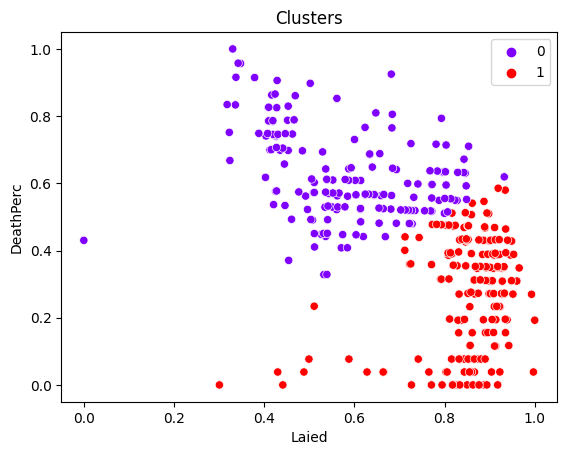
\includegraphics[width=70mm]
    {../Results/Two_clusters_division/CycleY/KMeans_scatter.png}}
         {K-means cluster scatter plot}
    \\
    \hline
    \subf{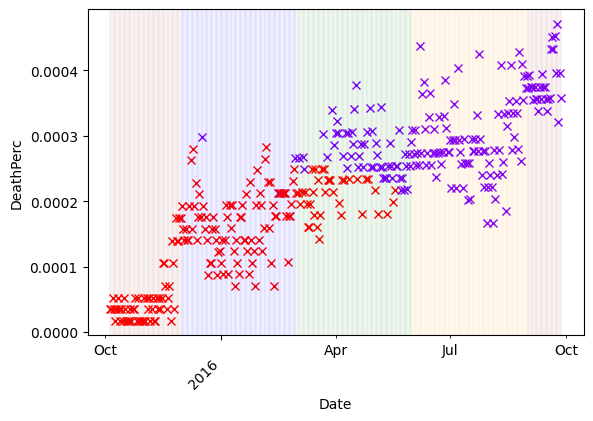
\includegraphics[width=70mm]
    {../Results/Two_clusters_division/CycleY/KMeans_plot_death.png}}
         {Percentage of death}
    &
    \subf{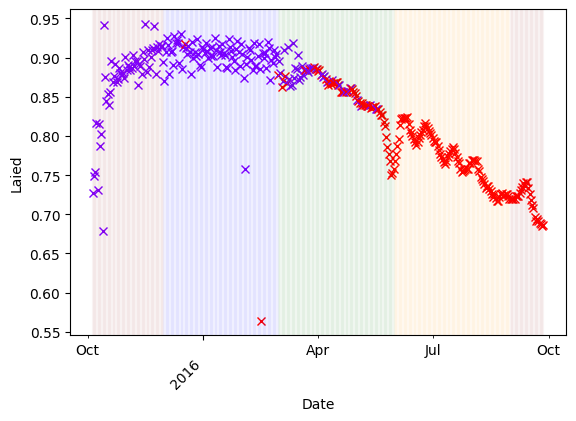
\includegraphics[width=70mm]
    {../Results/Two_clusters_division/CycleY/KMeans_plot_laied.png}}
         {Percentage of laid eggs}
    \\
    \hline
\end{tabular}
\end{center}

\subsection{Cycle Z}
\begin{center}
    \begin{tabular}{| c | c | c | c | c | c | c |} 
        \hline
        Arrival date & \#Chickens & Frist Laid & End of cycle & Organic & \#Eggs\\ [0.5ex] 
        \hline
        17/11/2016 & 42.130 & 08/01/2017 & 27/05/2018 & Yes & 17.721.240\\ 
        \hline
    \end{tabular}
\end{center}

Significant features:
\begin{itemize}
    \item Average Percentage of Laid Eggs each day: 87,78\%
    \item Average Percentage of Death each day: 0,021\%
    \item Average Temperature during the cycle: 13,07 °C
    \item Average Humidity during the cycle: 74,27\%
\end{itemize}

Cluster:
\begin{center}
\begin{tabular}{|c|c|}
    \hline
    \subf{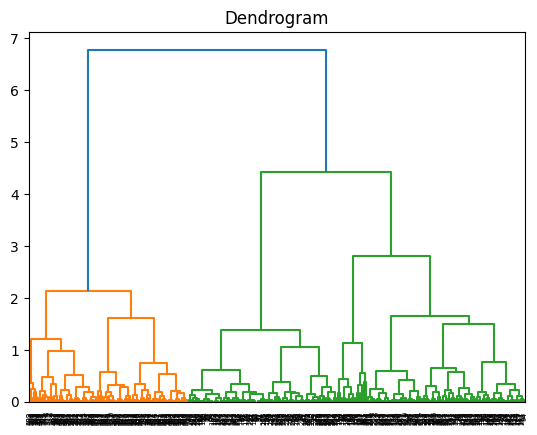
\includegraphics[width=70mm]
    {../Results/Two_clusters_division/CycleZ/Hierarchical_dendogram.png}}
         {Dendrogram}
    &
    \subf{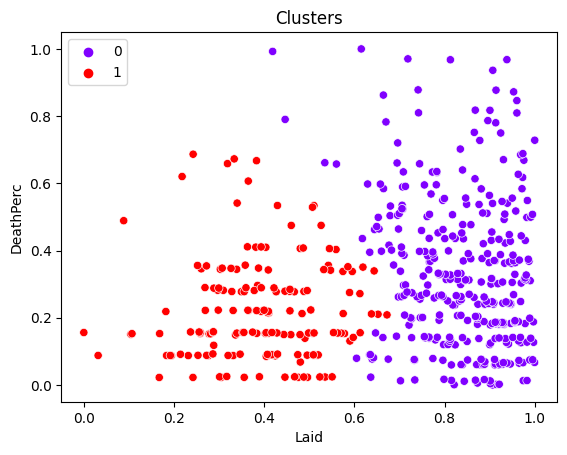
\includegraphics[width=70mm]
    {../Results/Two_clusters_division/CycleZ/Hierarchical_scatter.png}}
         {Hierarchical cluster scatter plot}
    \\
    \hline
    \subf{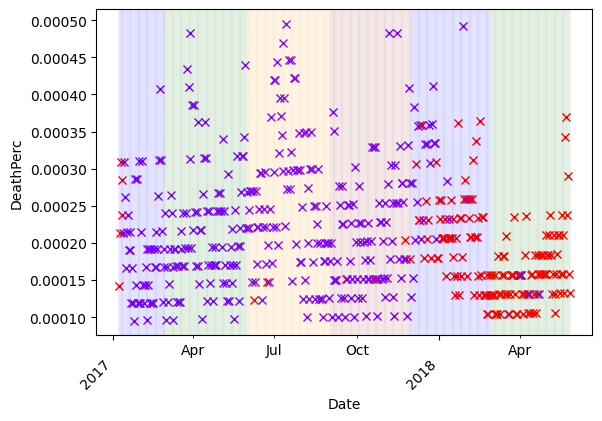
\includegraphics[width=70mm]
    {../Results/Two_clusters_division/CycleZ/Hierarchical_plot_death.png}}
         {Percentage of death}
    &
    \subf{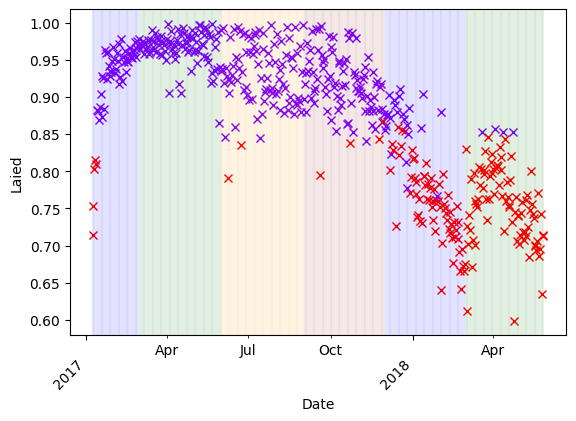
\includegraphics[width=70mm]
    {../Results/Two_clusters_division/CycleZ/Hierarchical_plot_laied.png}}
         {Percentage of laid eggs}
    \\
    \hline
\end{tabular}
\end{center}

\section{Common features}
In this section, we will discuss what we discovered by comparing all the cycles together.
After seeing that each cycle can be clustered in two parts, those clusters also divide the cycle into two distinct sections in a plot based on date. We tried to apply the same idea in a dataset composed of all the cycles together.

\begin{center}
    \begin{tabular}{|c|c|}
        \hline
        \subf{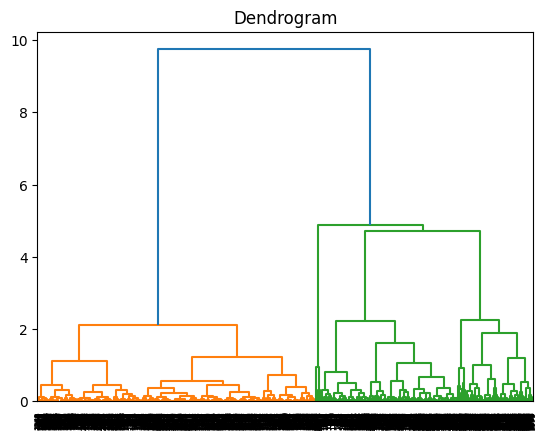
\includegraphics[width=70mm]
        {../Results/Every_cycle/Hierarchical_dendogram.png}}
             {Dendrogram}
        &
        \subf{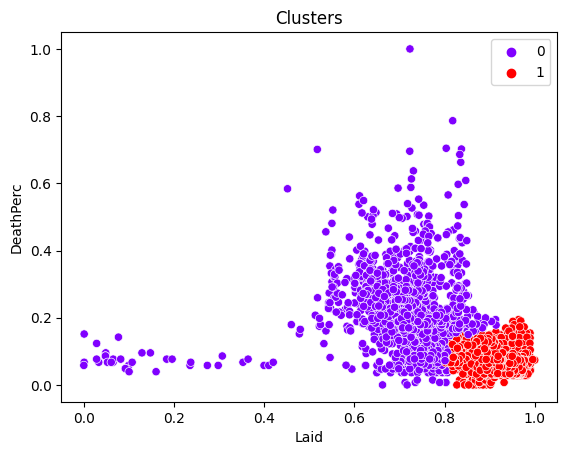
\includegraphics[width=70mm]
        {../Results/Every_cycle/Hierarchical_scatter_death.png}}
             {Hierarchical cluster scatter plot}
    \end{tabular}
    \begin{tabular}{|c|}
        \hline
        \subf{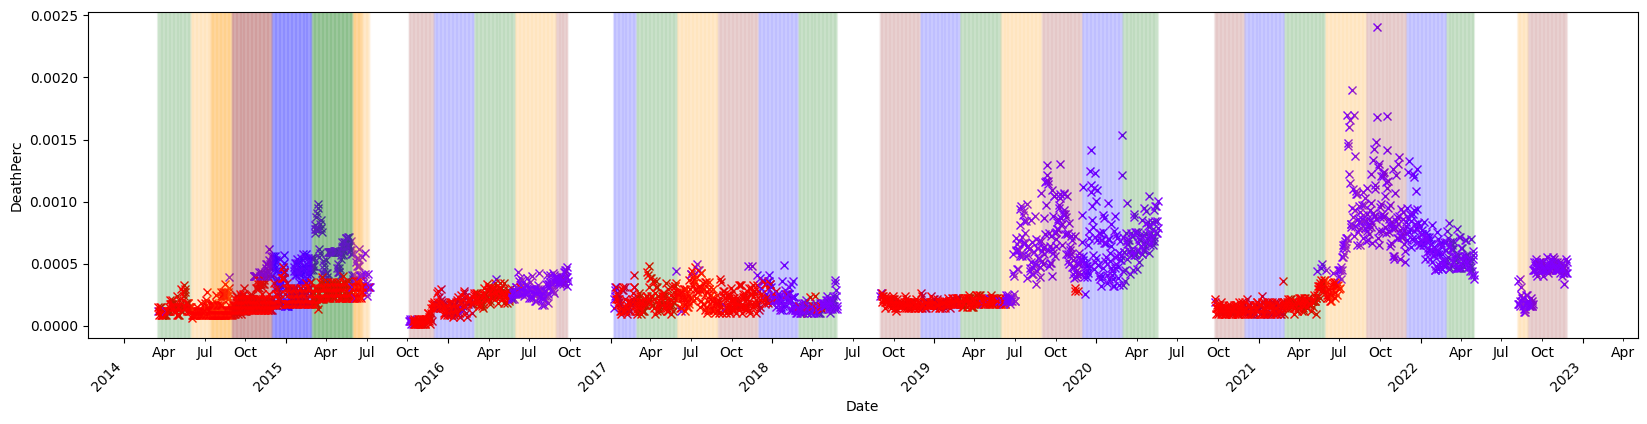
\includegraphics[width=144mm]
    {../Results/Every_cycle/Hierarchical_plot_death.png}}
         {Percentage of death}\\
    \hline
    \subf{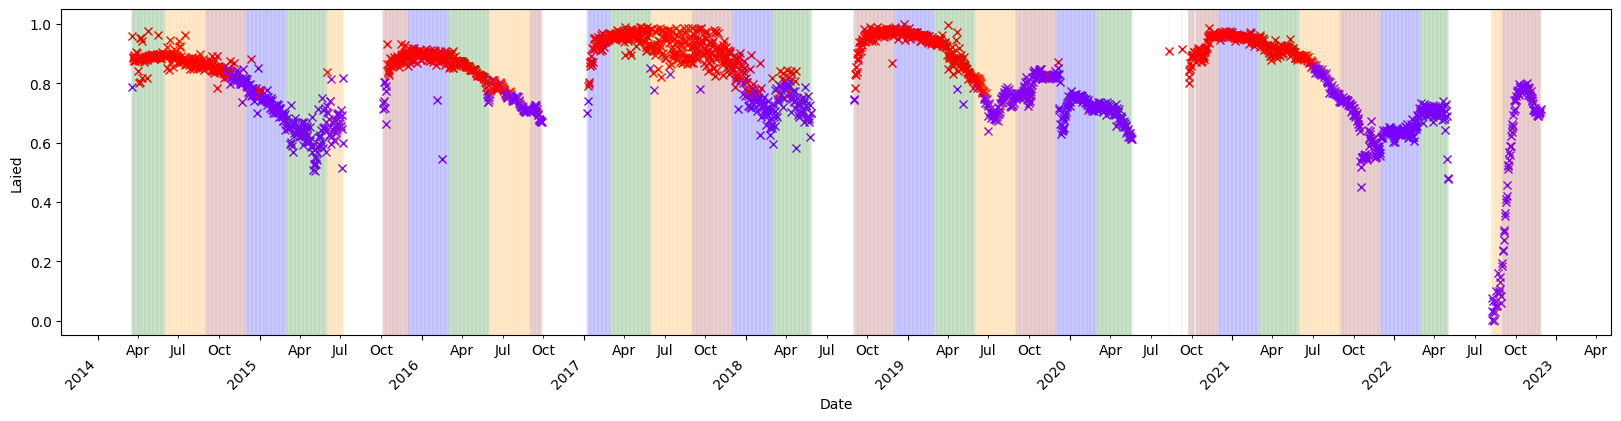
\includegraphics[width=144 mm]
    {../Results/Every_cycle/Hierarchical_plot_laied.png}}
         {Percentage of laid eggs}
    \\
    \hline
    \end{tabular}
    
\end{center}

Looking at the clusters we find that indeed the division of each cycle is respected. We find also that the only one that didn't respect this division is cycle C, which could be expected since it just started, but the interesting thing is that the whole cycle C is clustered as cluster 1 which is the one that identifies the end of every other cycle so we can see how bad is performing this new cycle both in death and laid rate.
This can show how the ban on beak-cutting affected the welfare of the chickens, with the beak the violence between animals increased a lot and not only increase the death rate but increased a lot the stress of the chickens reducing their productivity.

To better compare the different cycles we made a spider plot with 4 features:
\begin{itemize}
    \item Average Percentage of Laid Eggs each day
    \item Average Percentage of Death each day
    \item Average Temperature during the cycle
    \item Average Humidity during the cycle
\end{itemize}
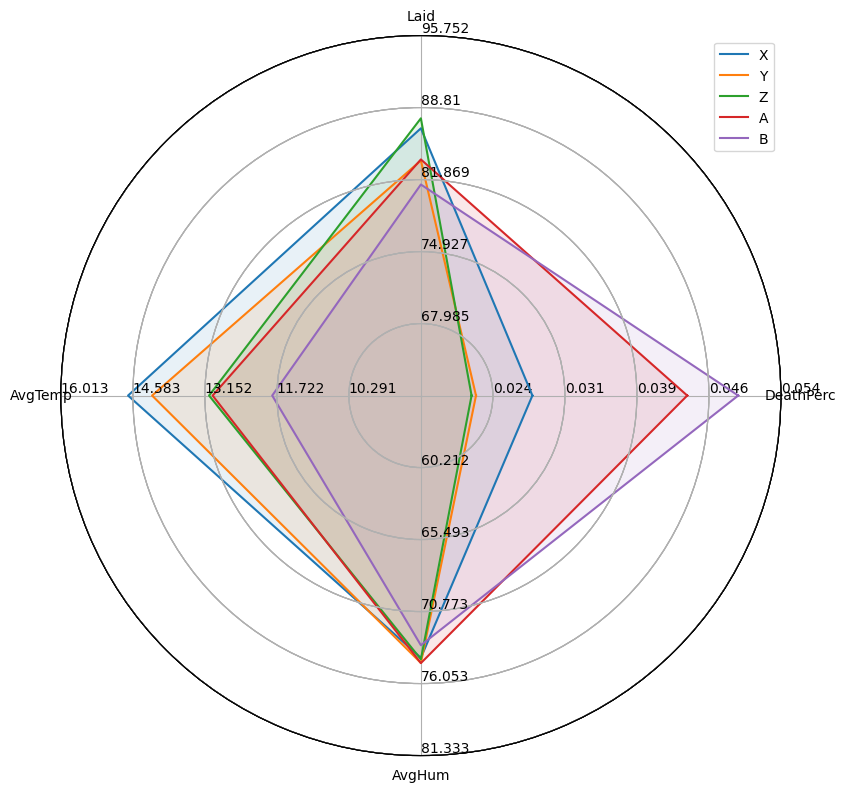
\includegraphics[width=\linewidth]{../Results/Every_cycle/Spider_Plot.png}


\section{Organic vs non-organic cycles}
One of the main differences in the cycles under analysis is the breeding method. Cycles A, B, C and Z are grown with organic farming, a method regulated by the European Union with the regulation 589/2008
modified from text 2168/2017 %da verificare e mettere fonte
while the cycles Y, X1 and X2 are non-organic.
We can summarize the main differences:

\begin{center}
    \begin{tabular}{| c | c | c |} 
        \hline
        Charachteristics & Organic & Non-organic \\ [0.5ex] 
        \hline
        Chickens$/m^{2}$ & 6 & 9 \\
        \hline
        Outdoor access & $\checkmark$ & $\checkmark$ \\
        \hline
        Feed requirements & $\checkmark$ & $\times$ \\
        \hline
    \end{tabular}
\end{center}

Given the differences in the breeding methods, we analyze if there are implications in the cycles' behavior. Since the non-organic ones have no information on feed and water consumption, we can't go
deep into the analysis because of the lack of inputs. For this reason, we will focus mainly on the outputs like the percentage of eggs laid and deaths.

One of the most important outputs is the productivity of a cycle expressed as EggsProduced\/\#Chickens. In the following results, we exclude cycle C since it is in progress. Furthermore, we round the 
data to the second digit.

\begin{center}
    \begin{tabular}{| c | c | c | c | c |} 
        \hline
        Cycle & Organic & Eggs per chicken & Breeding days & Productivity  \\ [0.5ex] 
        \hline
        A & $\checkmark$ & 481.04 & 627 & 0.84 \\ [0.5ex] 
        \hline
        B & $\checkmark$ & 436.90 & 586 &  0.81 \\ [0.5ex] 
        \hline
        Z & $\checkmark$ & 420.63 & 505 & 0.87 \\ [0.5ex] 
        \hline
        X1 & $\times$ & 366.77 & 478 & 0.80\\ [0.5ex] 
        \hline
        X2 & $\times$ & 316.29 & 342 & 0.95\\ [0.5ex] 
        \hline
        Y & $\times$ & 292.25 & 359 & 0.83 \\ [0.5ex] 
        \hline
    \end{tabular}
\end{center}

We can notice that non-organic cycles have a lower EggsProduced/\#Chickens rate than the organic ones, but considering the days of breeding the non-organic cycles are better.
The medium organic cycle productivity is 84\% while the non-organic one is 86\%.

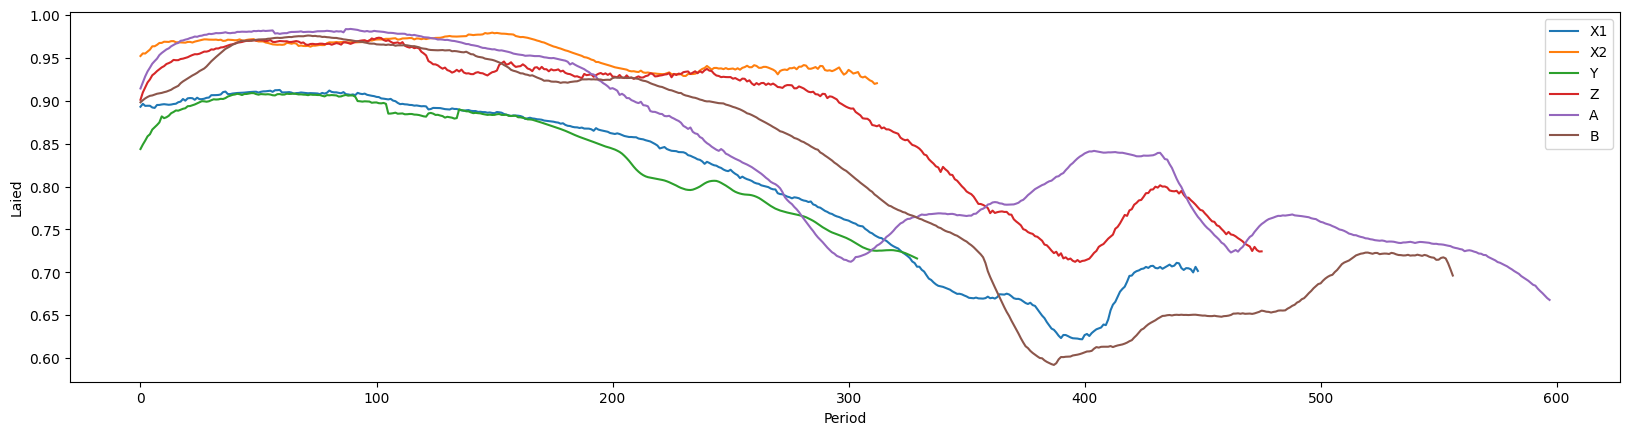
\includegraphics[width=\linewidth]{../Results/OrganingOrNot/Laid.png}

Beyond the productivity in terms of eggs produced there is another important aspect to consider which is the chickens' health. Since it is a difficult feature to value, 
we decided to consider the chickens' death percentage on the number of chickens as a health indicator.

\begin{center}
    \begin{tabular}{| c | c | c | c | c |} 
        \hline
        Cycle & Organic & Deaths on chickens & Breeding days & Daily deaths average \\ [0.5ex] 
        \hline
        A & $\checkmark$ & 0.24 & 627 & 16.18 \\ [0.5ex] 
        \hline
        B & $\checkmark$ & 0.25 & 586 & 18.07 \\ [0.5ex] 
        \hline
        Z & $\checkmark$ & 0.10 & 505 & 8.53 \\ [0.5ex] 
        \hline
        X1 & $\times$ & 0.14 & 478 & 10.10 \\ [0.5ex] 
        \hline
        X2 & $\times$ & 0.07 & 342 & 4.93 \\ [0.5ex] 
        \hline
        Y & $\times$ & 0.07 & 359 & 12.03 \\ [0.5ex] 
        \hline
    \end{tabular}
\end{center}

In organic cycles, the 'Daily deaths average' is higher than in non-organic ones: on average it is 5,76\% higher since it is 14.78\% in organic cycles and 9.02\% in non-organic ones.

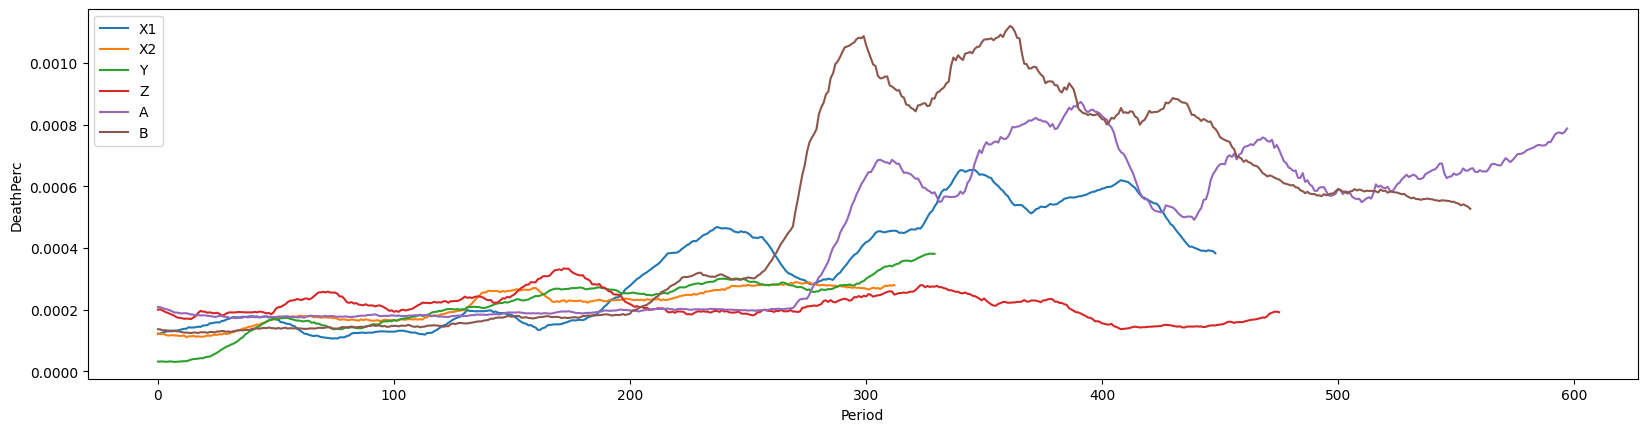
\includegraphics[width=\linewidth]{../Results/OrganingOrNot/DeathPerc.png}

Since non-organic cycles have both better productivity and a lower death rate it would be interesting to understand the reason. The parameters that could have an impact on this are various:
\begin{itemize}
    \item Alimentation: organic breeding has strict rules also in terms of feed
    \item Temperature: if a year is particularly hot chickens could suffer more
    \item Space: in organic cycles chickens have more space
    \item Time: the duration of a cycle could affect chickens' health
\end{itemize}

Since alimentation is one of the most important factors in the health of a living being and these data are missing in every cycle except for cycles A and B it could be difficult to answer the question
about chickens' health.
However, we tried to give some explanation based on our dataset and expert knowledge.

First of all, in almost every cycle, the correlation between the percentage of deaths and the period of breeding is high:
\begin{itemize}
    \item Cycle A: 0.73
    \item Cycle B: 0.63
    \item Cycle Z: -0.14
    \item Cycle Y: 0.86
    \item Cycle X1: 0.76
    \item Cycle X2: 0.68
\end{itemize}

The correlation with temperature is not as significant. If considered in the entire cycle, it becomes more interesting if it is considered just the part of the cycle in which the temperature rises.

...

\section{Death-season correlation}
In this section, we will analyze how the period when the chickens are introduced into the barn affects the mortality rate. This effect will be more visible in the organic cycles where the chickens are more fragile due to a lack of nutrients.

First, we plot the Death Rate of all the organic cycles (Z, A, B).\newline
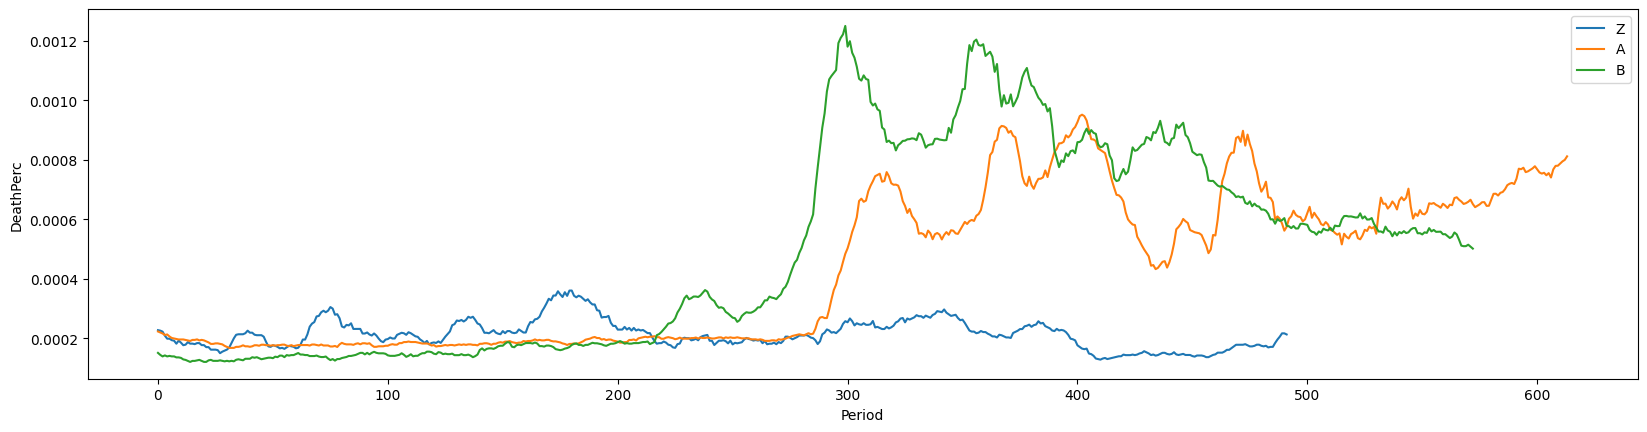
\includegraphics[width=\linewidth]{../Results/Comparison_Z_AB/Death.png}

It's clear that the Z cycle outperforms the other two by a lot, so we will analyze what are the differences between those 3 cycles.

The number of chickens at the start of the cycle is identical ($\sim 42.000$), and the feed in an organic farm is standard and checked so it doesn't change between those cycles.
The difference in mortality cannot be explained with just "a lucky cycle" so we tried to analyze those graphs deeper.
\begin{center}
    \begin{tabular}{|c|c|}
        \hline
        \subf{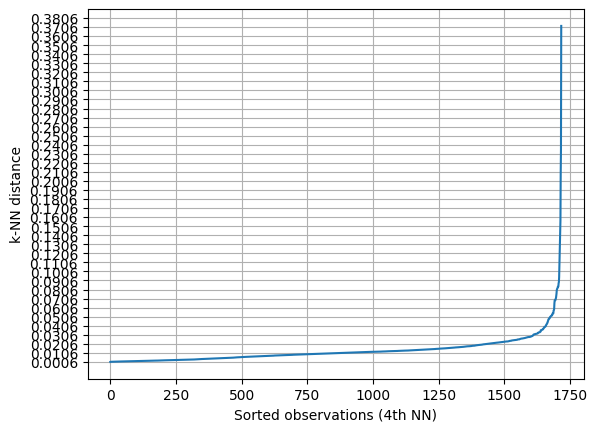
\includegraphics[width=70mm]
        {../Results/Comparison_Z_AB/Density_distance.png}}
             {k-NN distance to find $\epsilon$}
        &
        \subf{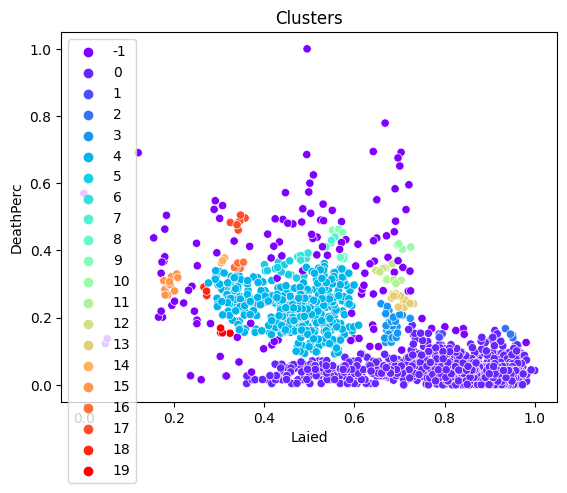
\includegraphics[width=70mm]
        {../Results/Comparison_Z_AB/Density_Raw.png}}
             {Raw Density}\\
        \hline
    \end{tabular}
    \begin{tabular}{|c|}
        \subf{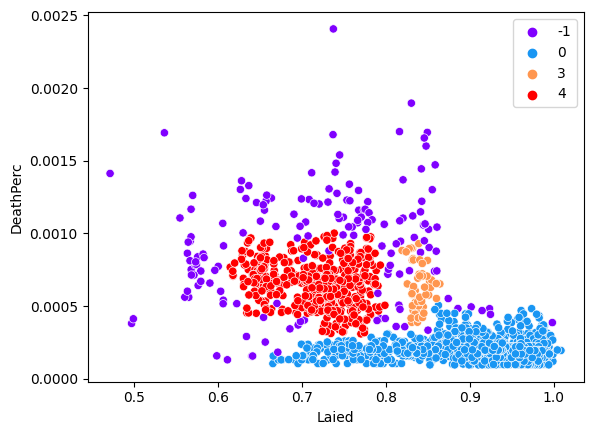
\includegraphics[width=70mm]
        {../Results/Comparison_Z_AB/Density_Cleaned.png}}
             {Density Cleaned}\\
    \end{tabular}
    \begin{tabular}{|c|}
    \hline
    \subf{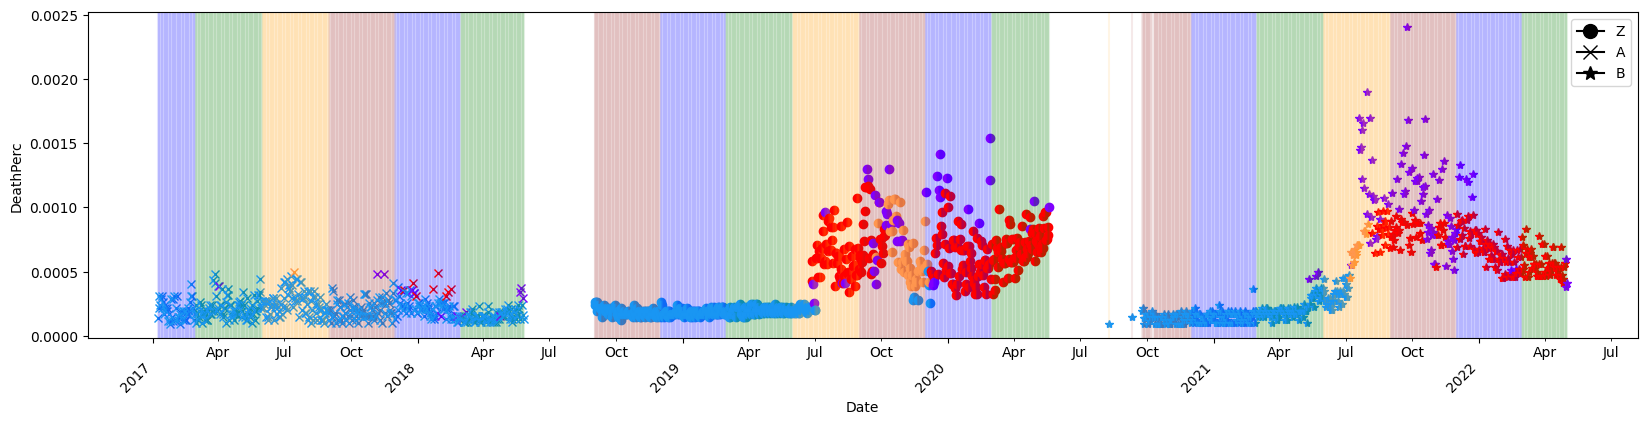
\includegraphics[width=144 mm]
    {../Results/Comparison_Z_AB/Plot_Clusters.png}}
         {Percentage of death}
    \\
    \hline
\end{tabular}
\end{center}

We see as expected that cycle Z is clustered the same as the start of the other cycles. But the interesting analysis is over the season in which events happen.

\begin{itemize}
    \item Both cycles A and B start to see an increase in mortality around mid-summer whereas cycle Z just saw a small peak.
    \item Cycles A and B started around early Autumn whereas cycle Z started in mid-winter
\end{itemize}

What also happens in the summer is that chickens start to eat less and so become weaker.

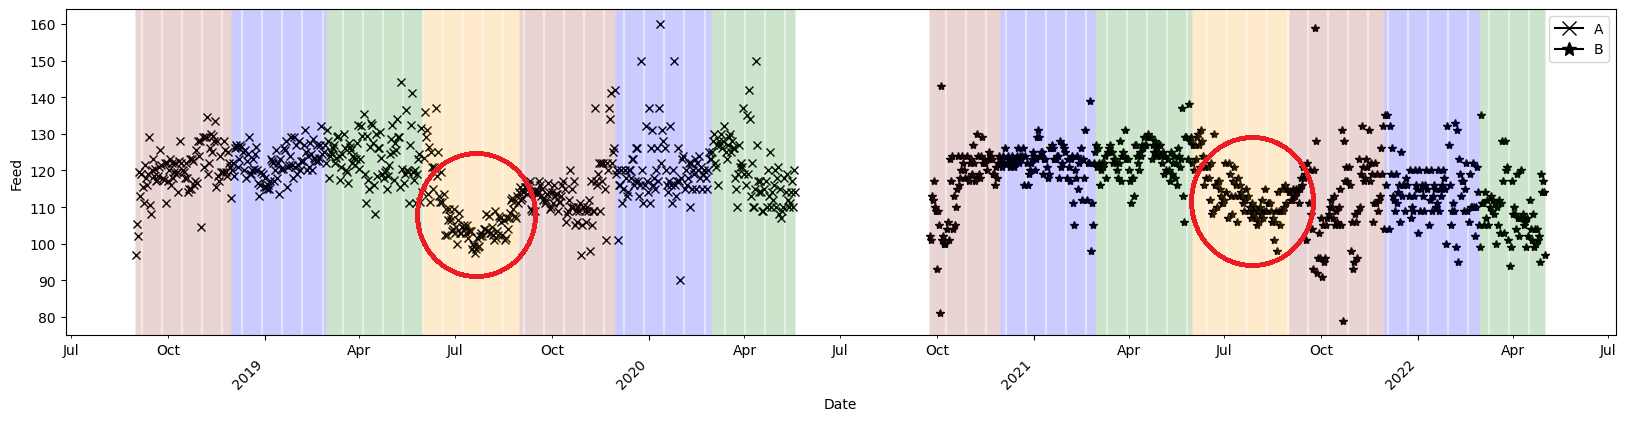
\includegraphics[width=\linewidth]{../Results/Comparison_Z_AB/feed_plot.png}

After discussing it with the farmer we conclude that the summer is the most challenging period for the chickens since:
\begin{itemize}
    \item The barns don't have air-conditioning and the Temperature can be quite high.
    \item The chickens are weaker due to age and the quality of nutrients in the organic feed.
\end{itemize}

To overcome those problems it seems that starting the cycle in mid-winter improves the mortality rate since during the summer the chickens are younger and stronger.

To put it in perspective, cycle Z had 4308 deaths compared to cycles A and B which had respectively 7449 deaths and 9130 deaths across the same period.
This help the production of cycle Z which, in the same period, produced 500.000 more eggs than cycle A and 1.200.000 more eggs than cycle B. Which is respectively an increment of 2\% and a 7\% in eggs produced.

\section{Cycle C}
Cycle C is a particular cycle, it is an organic cycle so it has the same characteristics as cycles A and B but from this one, a new regulation has been introduced. This new law banned the cut of the beak from the chick which increased the violence between the animals and this led to a higher mortality rate.\\
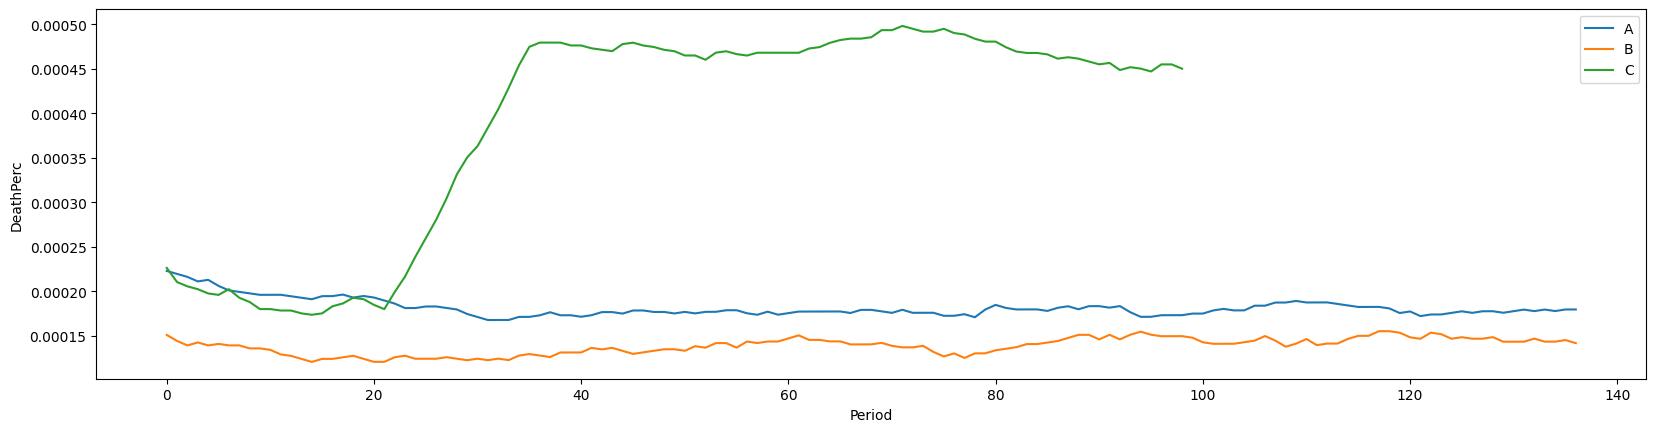
\includegraphics[width=\linewidth]{../Results/Comp_AB_C/Death.png}
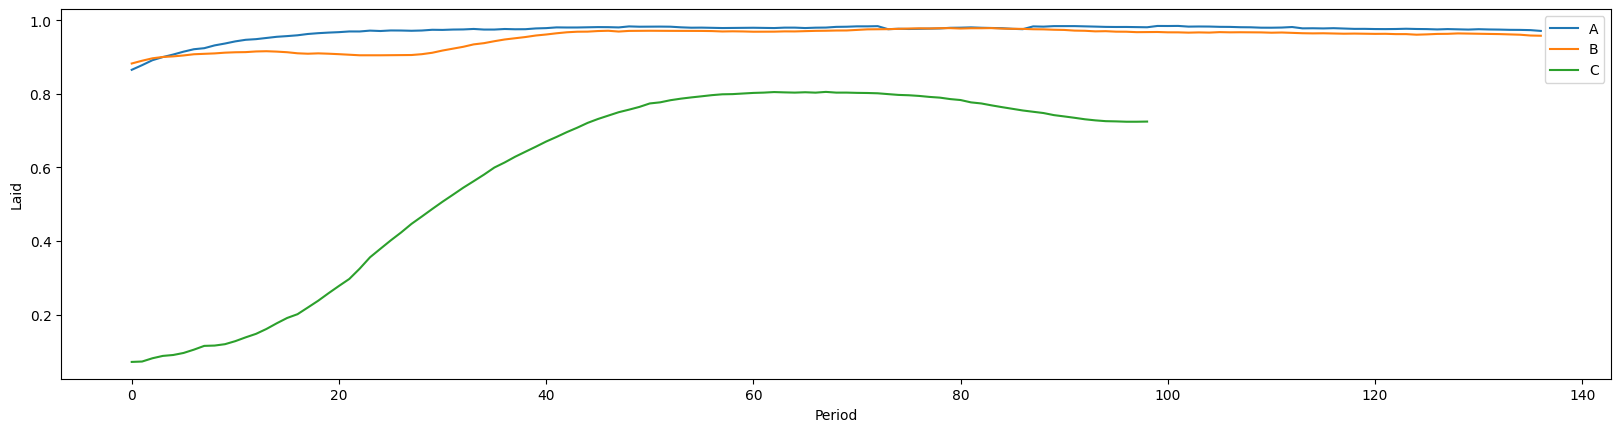
\includegraphics[width=\linewidth]{../Results/Comp_AB_C/Laid.png}

A difference of 0,03\% means on average that in this period every day die 12 chickens more than the normal rate.
This has an effect also on production since the chickens have poorer welfare they produce less.

Using a gradient boost regression we were able to guess the death that this cycle will have in the first 400 days based on the data that we have with the other 2 cycles A and B.\newline
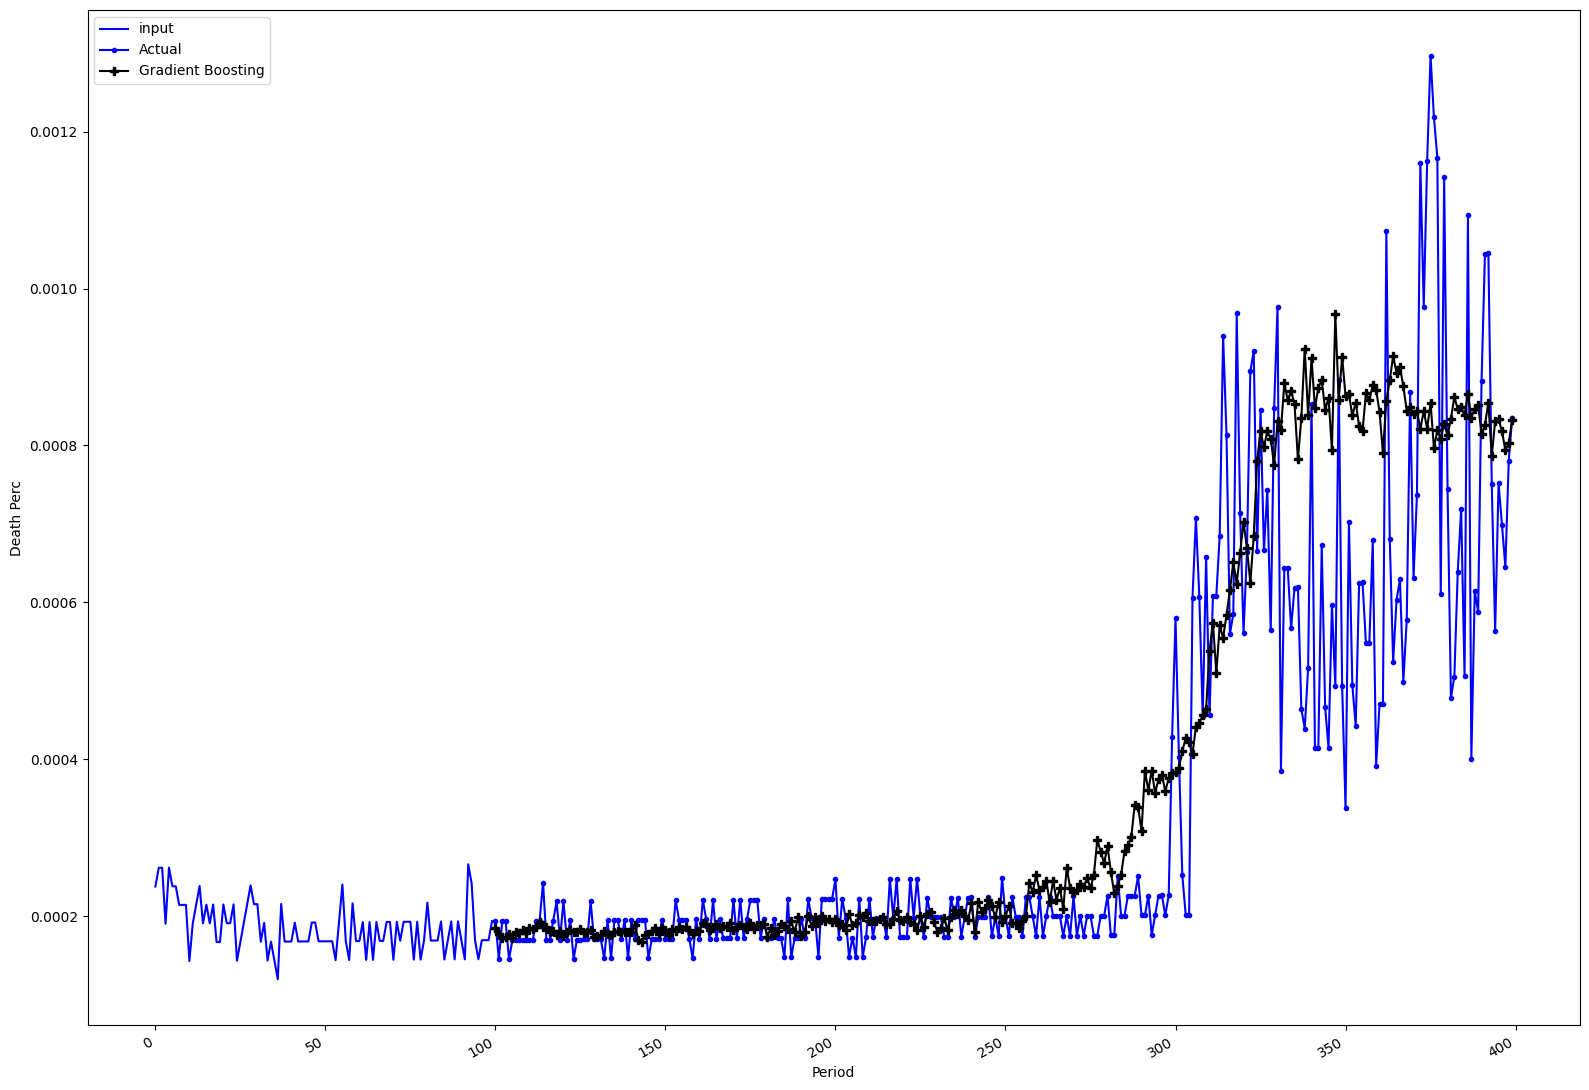
\includegraphics[width=\linewidth]{../Results/Comp_AB_C/predictor.png}
\newline
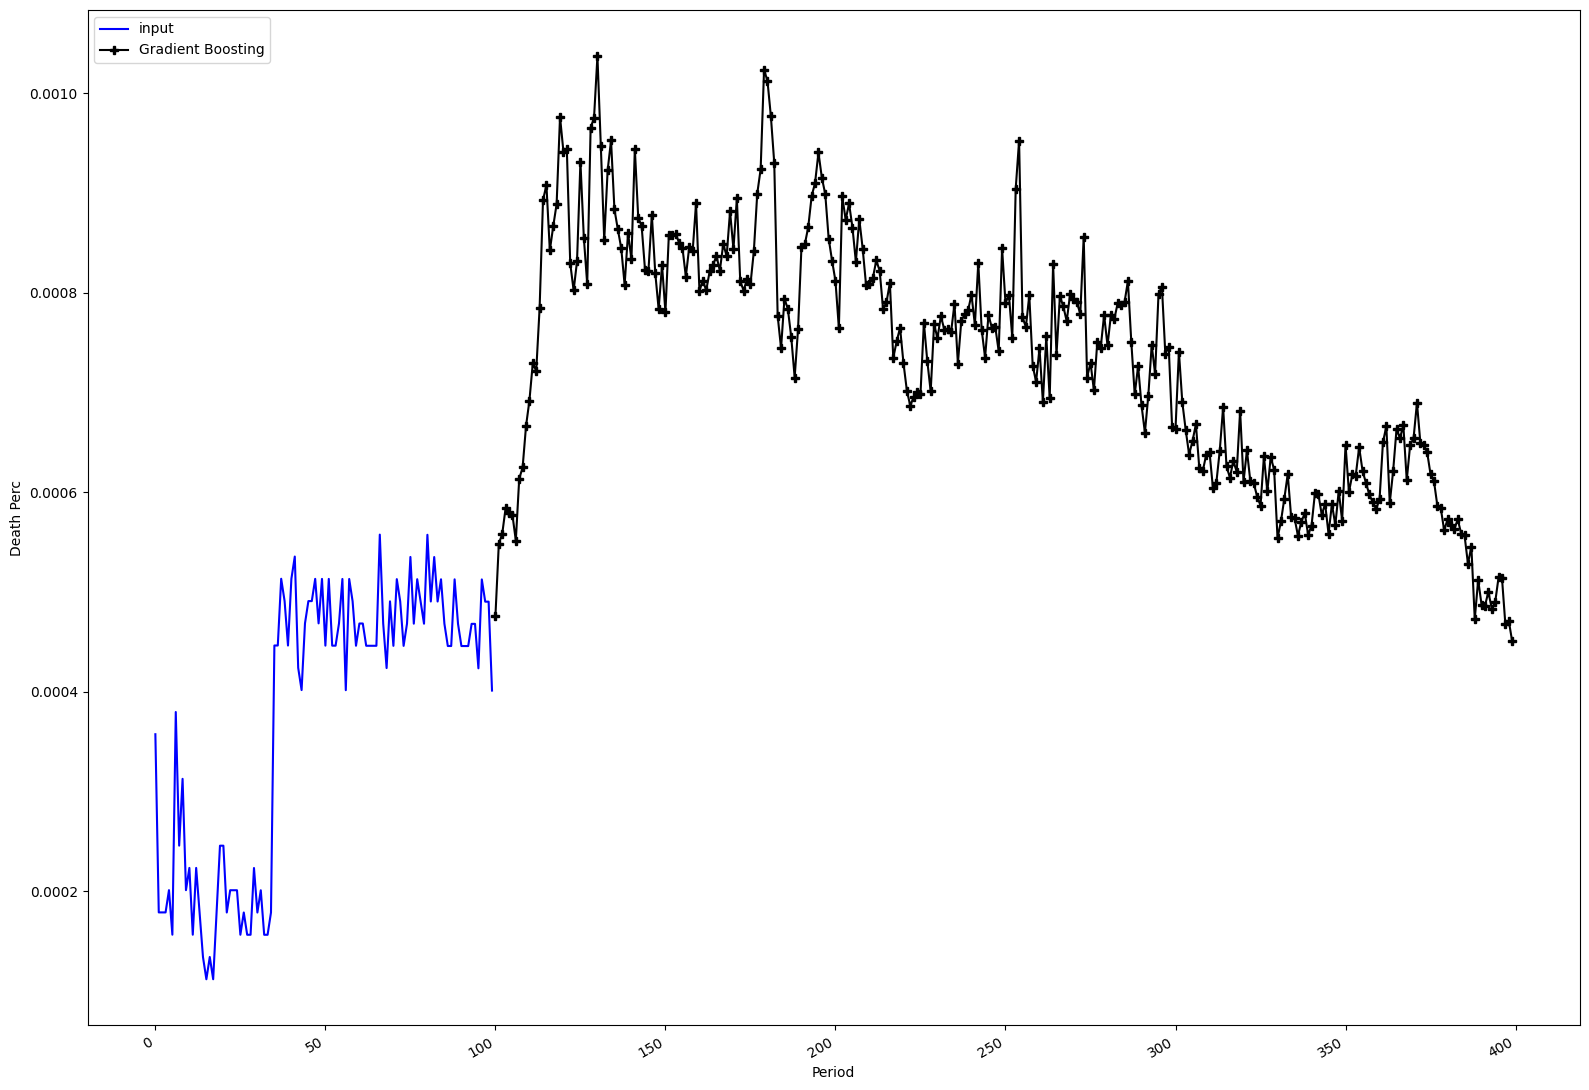
\includegraphics[width=\linewidth]{../Results/Comp_AB_C/predicted.png}

Using this prediction we say that we guess that in the first 400 days the farmer will lose 9210 compared to the 4903 of cycle A and 6369 of cycle B.

\section{Economic results}

\section{Data processing: shakiba}

\end{document}
